\section{Implementation}
\label{implementation}
The image processing is implemented in Matlab using the Computer Vision System Toolbox™. The implementation is built up as follows:
\begin{enumerate}
\item Image pre-processing before edge detection
\item Edge detection using the Canny algorithm
\item Hough transform to identify wall segments
\item Transformation from pixel coordinates to real life coordinates using GSD
\end{enumerate}

\subsection{Image pre-processing}
\begin{lstlisting}
%Read image
I = imread('ltest1.jpg');
%Resizing by a factor of 0.4
resize = 0.4;
I = imresize(I,resize);
%Nonuniform illumination correction
Ic = imcomplement(I);
%Morphological opening to estimate background
background = imopen(Ic,strel('disk',20));
%Subtract the background image from the original image
I2 = Ic - background;
%Convert image to gray-scale
I3 = rgb2gray(I2);
%Adjust the intensity values in the image (increase contrast)
I4 = imadjust(I3);
\end{lstlisting}
The initial processing done on the image is to make it easier to detect edges for the edge detection algorithm. Since we are dealing with very high resolution images (greater than 4k), we re-size the image to increase computation efficiency. This smooths the image, but this also has the potential to introduce a small error in the actual edge location, but this error is negligible for our application. \\

The method of correcting nonuniform illumination is not always required to make the Canny edge detection detect the important edges, but is important for the first order derivative edge detection algorithms. The \texttt{imopen} function morphologically opens the image with a disc-shaped structuring element of 20 pixels in radius. This is to estimate the nonuniform background illumination while not including the top of the wall. This value is then subtracted from the original image, and leads to more uniform illumination of the image.\\

The last step before edge detection is to convert the image from RGB to gray-scale. This is done by the function \texttt{rgb2gray}. This function eliminates the hue and saturation information of the image, while retaining the luminance. To increase the contrast of the image we adjust the intensity values in the image such that 1\% of the high and low intensity values are saturated with the function \texttt{imadjust}.

\subsection{Edge detection}
\begin{lstlisting}[firstnumber=16]
%Apply the Canny edge detection algorithm with the tuned
%threshold of 0.78
BW2 = edge(I4,'canny',0.78);
%Resize the image back to the original size for mapping
BW3 = imresize(BW2,(1/resize));
\end{lstlisting}
As mentioned earlier, the threshold value is an empirically determined value. This is in reality an upper and lower threshold where \texttt{edge} ignores all values that are not in between the upper and lower threshold. In the Canny algorithm, the threshold is a two-element vector where the upper threshold is the input value $0.78$ and the lower threshold is $0.4 \times$ upper threshold. There is also a possibility of specifying a $\sigma$ value for the Canny algorithm, where $\sigma$ is the standard deviation of the Gaussian filter in (\ref{gauss}).\\

The last step before applying the Hough transform is to re-size the image back to its original size, so that the edge segments and the lengths detected by the Hough transform is in the original image size.

\subsection{Hough Transform}
\begin{lstlisting}[firstnumber=21]
%Compute Standard Hough Transform of the image BW3.
[H,theta,rho] = hough(BW3);
%Locate peaks in the Hough transform matrix, H, generated by the hough 
%function. The second input value specifies the maximum number of peaks
%(lines) to identify
P = houghpeaks(H,6,'threshold',ceil(0.1*max(H(:))),'NHoodSize',[9,9]);
%Extract line segments in the image BW3. Returns structure array
%whose length equals the number of merged line segments found.
lines = houghlines(BW3,theta,rho,P,'FillGap',600,'MinLength',900);
\end{lstlisting}
This is the basic implementation of the Hough transform in Matlab. It starts by computing the Standard Hough Transform by using the parametric representation of a line 
\begin{align*}
\rho=x\cos{\theta} + y\sin{\theta}
\end{align*}
as explained in Chapter \ref{ch:hough}. \texttt{hough} returns theta $(\theta)$, rho $(\rho)$ and H. Theta and rho are the arrays of rho and theta values over which the Hough transform matrix H was generated. The next step is to find the peaks in the Hough transform matrix H. \texttt{houghpeaks} is used for this purpose and can be modified to find the important line segments. The function takes in a threshold which is the minimum value to be considered a peak in H. \texttt{NHoodSize} is the neighborhood around each peak that is set to zero after the peak is detected by the algorithm. This value has to be an odd-number. We can also define the maximum number of peaks we want to detect.\\

Th next step is to extract the line segments from the binary edge detected image based on the Hough transform. \texttt{houghlines} takes in the the binary edge detected image, and the values computed by the Hough transform. In addition we can define \texttt{FillGap} and \texttt{MinLength} which is used to connect edges and suppress edges below a minimum length respectively. Based on the peaks found in the Hough transform the function searches for line segments, and returns a structure array whose length equals the number of merged line segments identified.\\

We can display the Hough transform matrix H to illustrate the relationship of $\rho$ and $\theta$ in the image by using the following code. This is the H matrix of the image used when determining the ideal edge detection algorithm; \texttt{Compare.jpg} in Figure \ref{fig:testimage}.
\begin{lstlisting}[firstnumber=30]
%Display H matrix image of Compare.jpg
imshow(imadjust(mat2gray(H)),'XData',theta,'YData',rho, ...
	'InitialMagnification','fit');
title('Hough transform of Compare.jpg');
xlabel('\theta'), ylabel('\rho');
set(gca,'fontsize',20);
axis on, axis normal, hold on;
\end{lstlisting}
\begin{figure}[H]
\centering
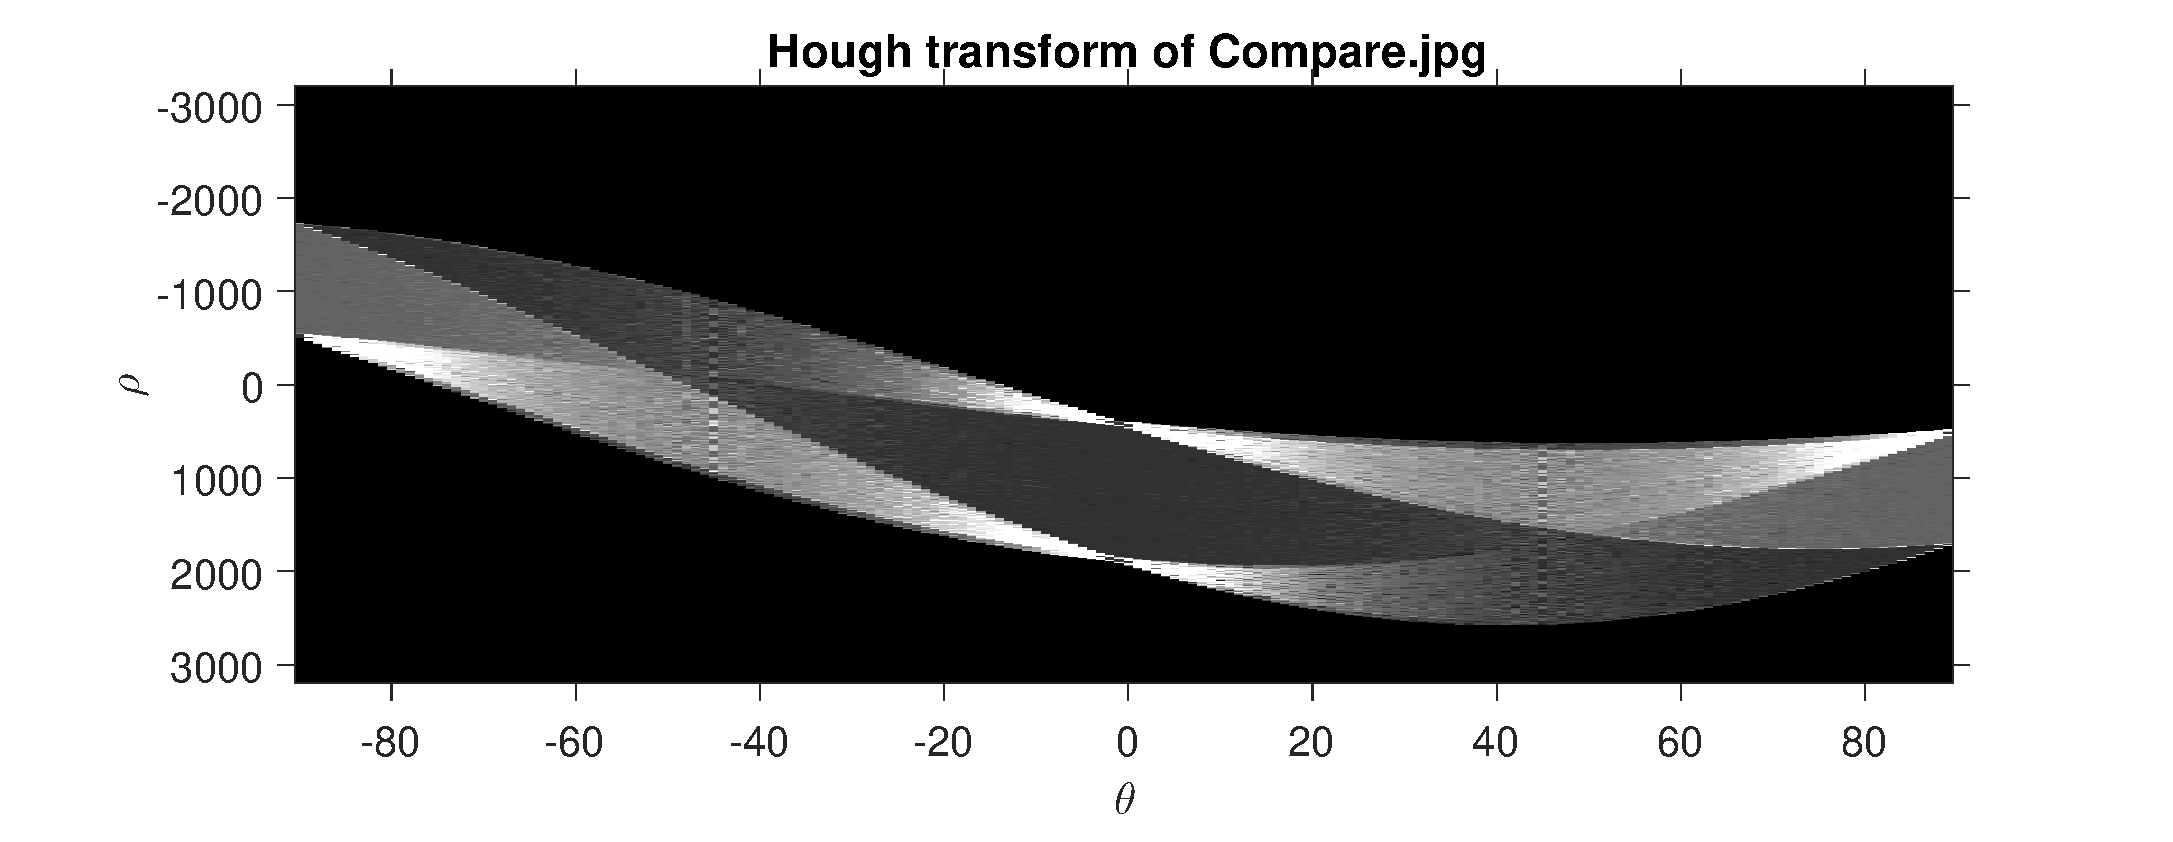
\includegraphics[width=\textwidth]{fig/houghcompare}
  \caption{Hough transform matrix M}
  \label{fig:houghcompare}
\end{figure}

Since we now have the line segments detected in the image, we can now compute the lengths and plot the lines over the original edge detected binary image. The computation of lengths is needed for the implementation of transforming the lengths from pixel values to real life meter values. 

\begin{lstlisting}[firstnumber=37]
%Display the edge detected binary image BW3
figure,imshow(BW3), hold on

for k = 1:length(lines)
	%Iterate over every x-y coordinate in lines
	xy = [lines(k).point1; lines(k).point2];
    
    %Plot every line segment found previously
    plot(xy(:,1),xy(:,2),'LineWidth',3,'Color','green');
   	
   	%Plot beginnings and ends of lines
   	plot(xy(1,1),xy(1,2),'x','LineWidth',2,'Color','yellow');
   	plot(xy(2,1),xy(2,2),'x','LineWidth',2,'Color','red');    
    
   	%Compute length of each line segment and store in lengthlines(k)
   	lengthlines(k) = sqrt((xy(2,1)-xy(1,1))^2 + (xy(2,2)-xy(1,2))^2);
    
   	%Display length of each line segment
   	text(xy(1,1),xy(1,2), [int2str(lengthlines(k)),'------'], ...
   	'Color','red','HorizontalAlignment','right')    
end
\end{lstlisting}
Using the same test image, \texttt{Compare.jpg} after edge detection and Hough transform this implementation will output the following image of the edge detected image with the Hough transform lines overlay:

\begin{figure}[H]
\centering
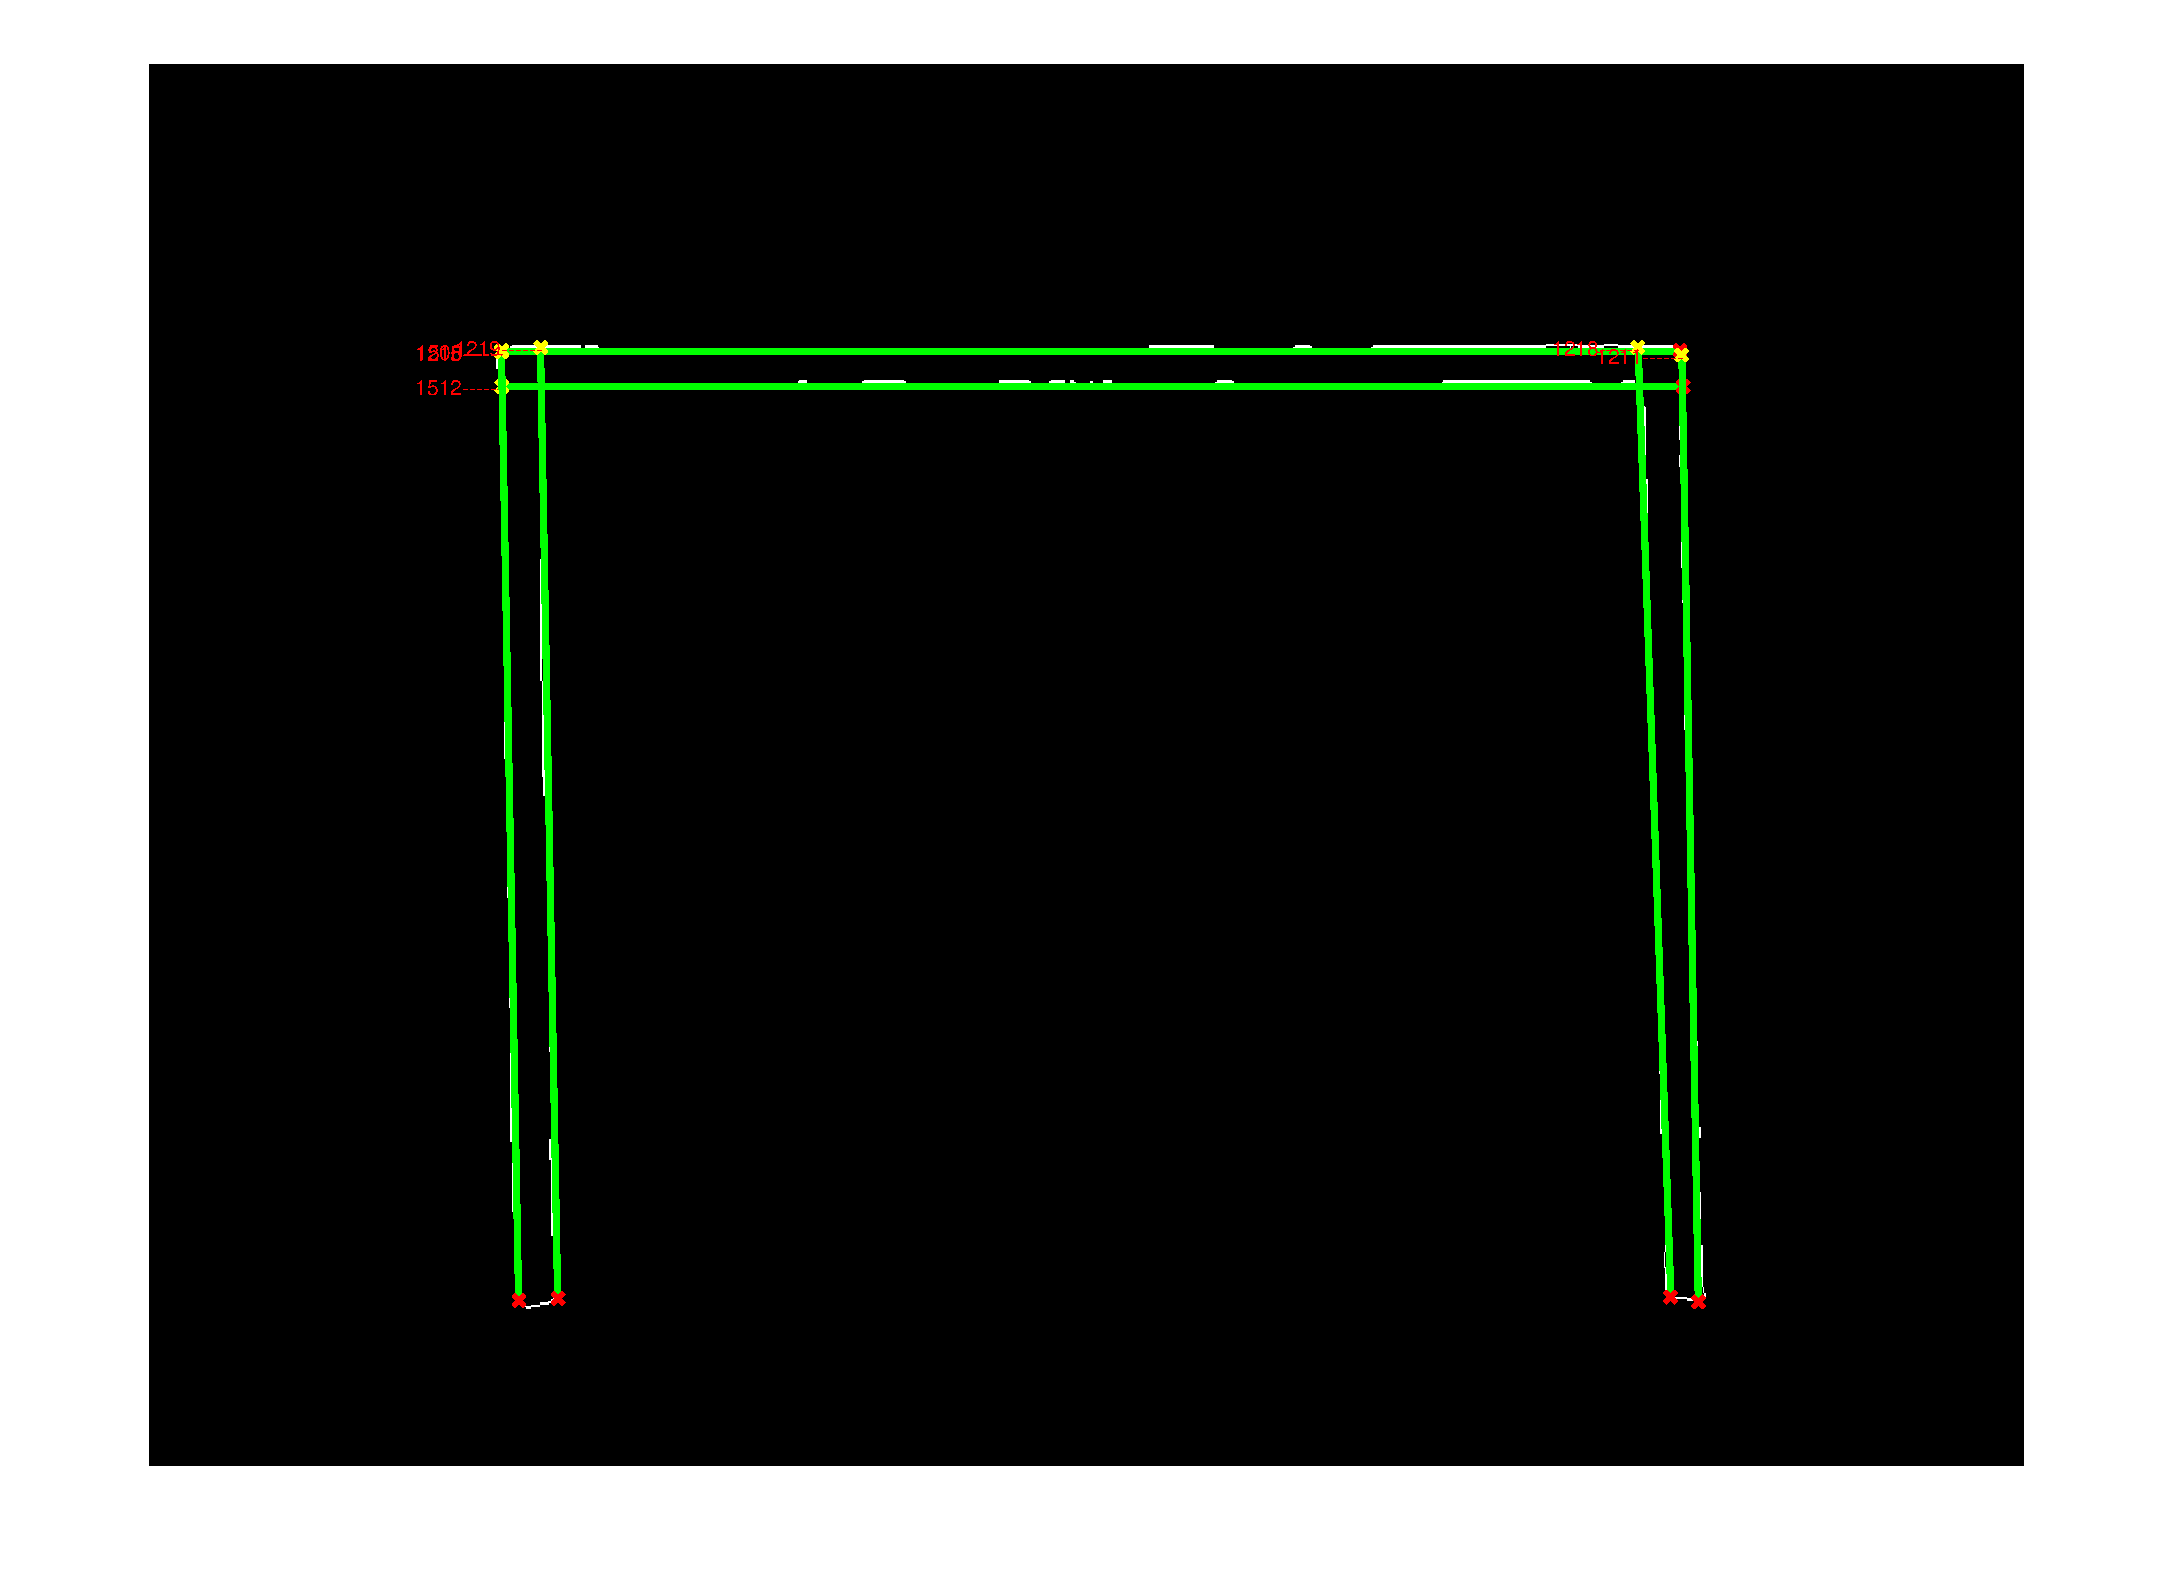
\includegraphics[width=\textwidth]{fig/lines}
  \caption{Hough transform overlay}
  \label{fig:houghcompare}
\end{figure}

\subsection{Transformation of pixel values}
Section \ref{ch:mapping} covers the theory of our implementation to transform the pixel values to real life values with respect to the location of the image sensor. The first step of this transformation is to calculate the GSD:
\begin{lstlisting}[firstnumber=58]
%Calculate GSD
Sw = 6.17; %Sensor width of image sensor [mm]
Fr = 4.67; %Focal length of image sensor [mm]
H = 1.06;  %Heigth of image sensor (to wall) [m]
Iw = 4000; %Image width [pixels]
Ih = 2992; %Image height [pixels]
GSD = (Sw*H*100)/(Fr*Iw); %GSD in cm/pixel
\end{lstlisting}
The test image \texttt{Compare.jpg} is cropped uniformly around the center, while the values for image width and image height is based on the original image taken. This does not move the center, which means we can use the GSD from the original image after cropping.\\

We define the center of the image:
\begin{lstlisting}[firstnumber=65]
%Define the center of the image
[row, col] = size(BW3);
x_center = col/2;
y_center = row/2;
c = [x_center; y_center];
\end{lstlisting}
The next step is to convert the pixel units to real life units. We have all the information we needed to calculate the length and position of the walls. Using the method described in Section \ref{ch:mapping}:
\begin{lstlisting}[firstnumber = 70]
figure, hold on

for k = 1:length(lines)
    %Find the real length of lines
    reallines(k) = GSD*(lengthlines(k));
    
    %Find the real coordinates of start- and end points
    %with respect to the image center
    xyreal = GSD*[lines(k).point1-[c(1),c(2)]; lines(k).point2-[c(1),c(2)]];
    
    %Plot the lines
    plot(xyreal(:,1),xyreal(:,2),'LineWidth',3,'Color','green');
    
    %Mark the length of each line 
    text(xyreal(2,1),xyreal(2,2),[num2str(reallines(k)),'cm'], ...
    'Color','red','Rotation','-45','Fontsize',12);   
end

%Setting plot variables 
set(gca,'fontsize',15,'ydir','reverse');
title('Location of walls with respect to image sensor');
xlabel('cm'), ylabel('cm');
%Plot center of image
plot(0,0,'x');
hold off
\end{lstlisting}
This for loop can be implemented in the same loop as the Hough transform algorithm, but for clarity they are separated for this implementation description. The code will produce a mapping of the walls detected relative to the image sensor position.

\begin{figure}[H]
\centering
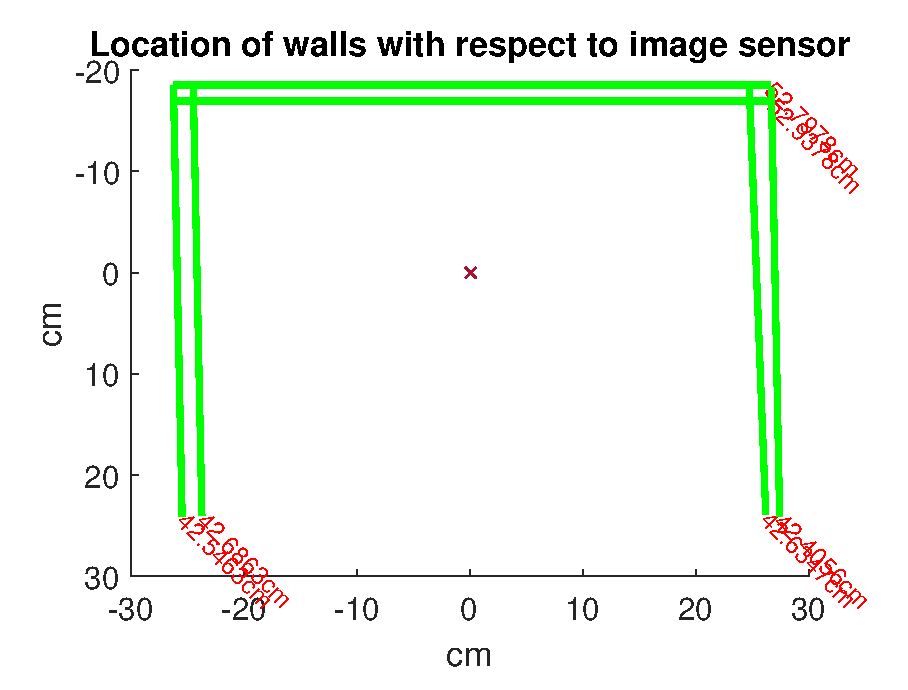
\includegraphics[width=\textwidth]{fig/mapping}
  \caption{Mapping of the walls relative image sensor in [cm]}
  \label{fig:mapping}
\end{figure}
We now have a complete mapping of the test maze in real life units with respect to the xy-position where the image was taken on the wall plane. The reason the y-axis is reversed is because the y-axis of the original image is measured from the bottom to the top, which is the inverse of the \texttt{plot} function. 



















